\section{Results/Analysis}

\subsection{Comparison between frameworks}
To compare between CNN frameworks, AlexNet was trained for many iterations on each framework.
The whole process was profiled, and one mini-batch iteration was selected for analysis after the time metrics were stabilized.
Model parameters and hyperparameters of the solver are carefully equalized previously in order to remove the effect from things other than the framework itself.
The result is shown in Figure~\ref{fig_time_frameworks}.

\begin{figure*}
  \centering
  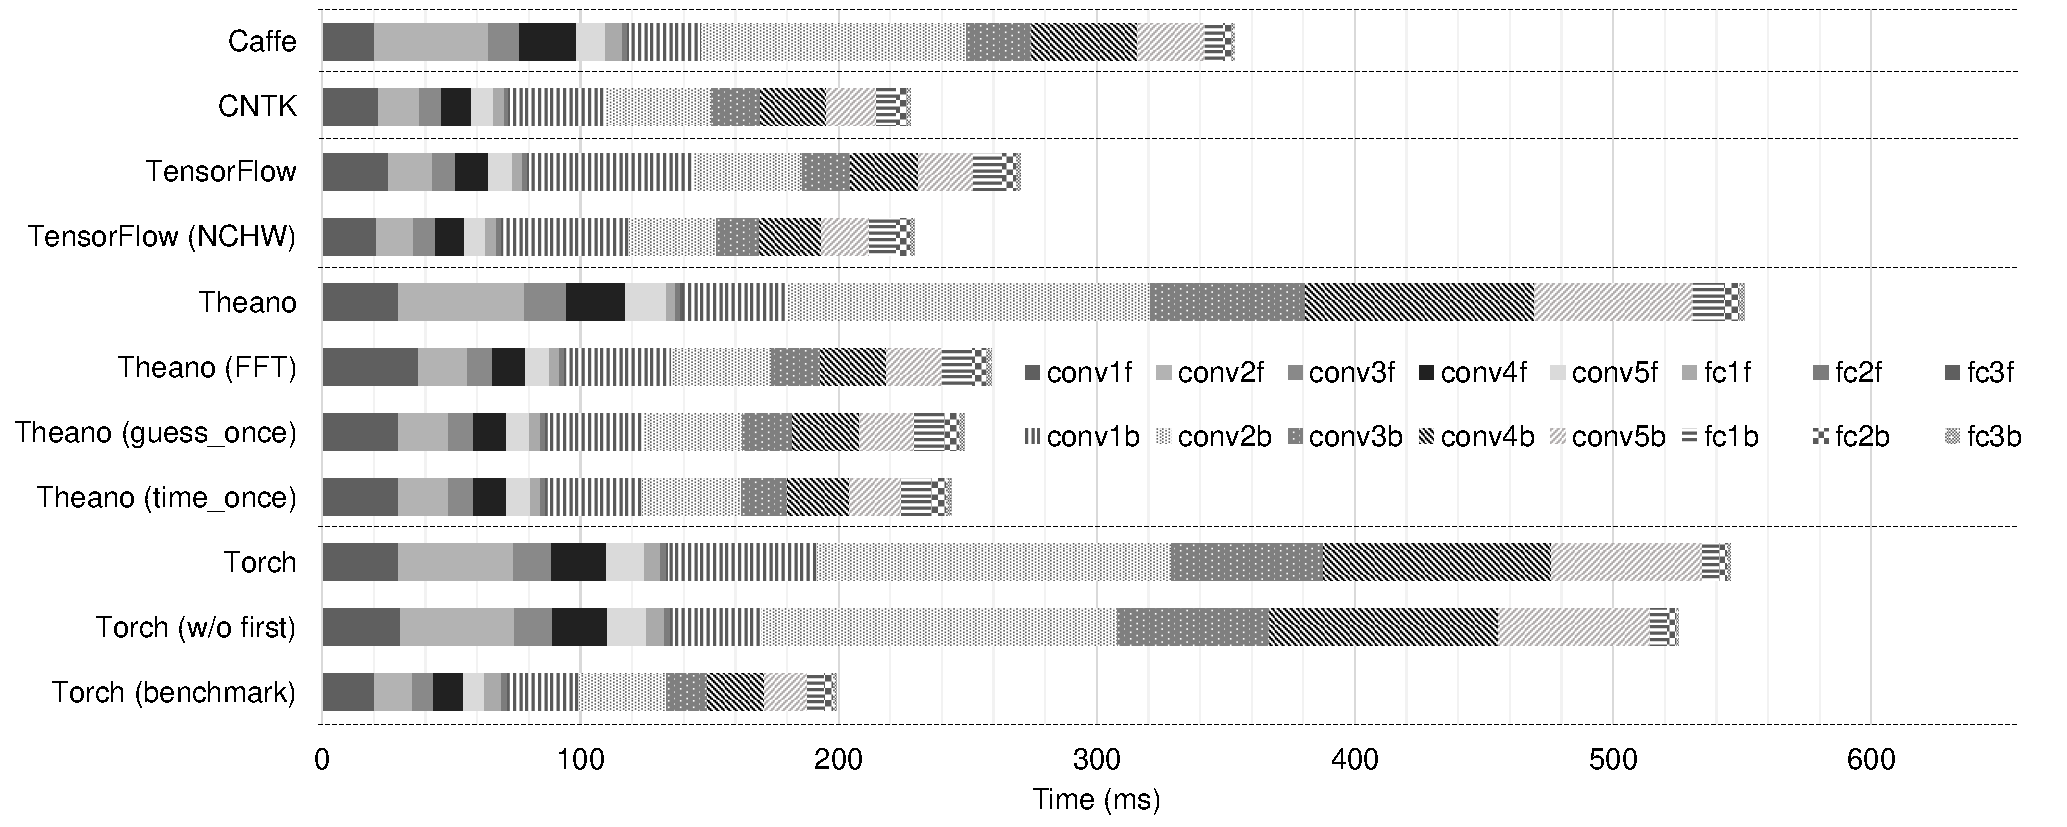
\includegraphics[width=\linewidth]{./figures/time_frameworks}
  \caption{
Layer-wise time of AlexNet training under various framework configurations.
In the legend, `conv' means convolution layer and `fc' means fully-connected layer.
Numbers mean the layer order in AlexNet.
Suffix `f' means forward propagation, and `b' means backward propagation.
Each alphabet means the following: A = Caffe, B = TensorFlow (default), C = TensorFlow (with NCHW tensor format), D = Theano (default), E = Theano (FFT), F = Theano (guess\_once), G = Theano (time\_once), H = Torch (default), I = Torch (no backward data convolution in the first layer), J = Torch (FFT), K = Torch (benchmark option).
}
  \label{fig_time_frameworks}
\end{figure*}

First, we focused at how each framework chose kernels.
Caffe did not provide any user options to affect kernel choices.
Instead, Caffe depended on cuDNN's heuristics, which try to determine the best suited algorithm under the given specification.
Surprisingly, Caffe did not have appropriate memory strategy for kernels yet, just passing 8MB workspace limit as an argument.
Low-memory required algorithms, such as gemm and winograd, were selected, resulting in low performance compared to other frameworks.
Tensorflow also did not provide options for kernel choices.
Unlike Caffe, however, it executed all available algorithms on the first run by itself.
Only the fastest kernels in each layer were executed for subsequent runs.
Under the AlexNet, FFT algorithms were chosen for all convolution layers except the first layer, where FFT cannot be used due to stride of 4.
One downside was that algorithms were chosen from hardcoded set, so recently added option (like WINOGRAD\_NONFUSED) was not included.

On the other hand, Theano provide full access on the kernel choices.
We could specify convolution algorithms to be used, globally or layer-by-layer.
We found layerwise option is better, since implicit gemm is chosen as fallback if the layer specification does not match global option, and it can even be slower than explicit gemm which is the default option.
This is the reason why the first layer of E in Fig~\ref{fig_time_frameworks} is slower than F, G, and even D.
Theano also had `guess\_once' option, which depended on cuDNN's heuristics like Caffe but provided proper arguments.
`time\_once' option was provided, too, which depended on cuDNN's functionality that run all available convolution algorithms and chose the fastest one.
Theano did not have downside like TensorFlow had, because it directly used cuDNN's API.
If `time\_once' option was on, it used gemm on the first layer and had mixed use of FFT and winograd on the rest convolution layer.
When `guess\_once' option was on, it used slightly different kernels but showed almost identical running time with `time\_once' option, proving that heuristic of cuDNN is quite reliable.
Although Theano executed the fastest convolution kernels, Theano did not have the fastest convolution when it came to the whole layer.
Theano used its own runtime-compiled kernels for bias add and ReLU activation, and they were more than twice slower than cudnn's or other libraries'. (Table~\ref{table_misc_kernel})
Torch provided full control on the kernel choices, similar to Theano.
Torch's cuDNN backend, cudnn.torch had cudnn.benchmark option which is the same with `time\_once' in Theano.
When benchmark option is on, Torch showed overall fastest execution time among four frameworks.

\begin{table*}[]
\centering
\caption{misc. kernels}
\label{table_misc_kernel}
\begin{tabular}{llllll}
\multicolumn{2}{l}{Framework} & Caffe & TensorFlow & Theano & Torch \\ \hline
Bias addition    & From       & cuDNN & TensorFlow & Theano & cuDNN \\
                 & Time (ms)  & 2.64  & 2.84       & 7.88   & 2.63  \\
ReLU activation  & From       & cuDNN & Eigen      & Theano & cuDNN \\
                 & Time (ms)  & 2.56  & 2.43       & 4.59   & 2.56 
\end{tabular}

This table is about kernels included in convolution layers, but not directly participating in convolutions.
`From' means which library kernels came from.
Times are measured in the first convolution layer.
Noticeably, Theano uses kernels which are compiled in runtime and they are quite slow compare to others.
\end{table*}

We also found a few phenomenons in terms of framework overhead.
The most noticable one was the tensor format.
Caffe, Theano, and Torch used NCHW tensor format, which means (batch, channel, height, width) dimensions.
Tensorflow supported NCHW, but it used NHWC more popularly.
Its tutorial codes used NHWC format, and many functions, like conv2d, used NHWC as a default argument.
While NHWC can be faster when there are channel-wise operations, some cuDNN's convolution kernels (such as FFT) only support NCHW format.
Besides, TensorFlow always do NHWC-to-NCHW dimension swap even if it is using NHWC-supported kernels.
Therefore, using NHWC tensor format leads to intensive dimension swapping before and after the convolution.
In our AlexNet, just changing tensor format from NHWC to NCHW led to about 15\% improve in speed on TensorFlow.
Second issue was backward data convolution in the first convolution layer.
The first layer does not have previous layer to update parameters, so it does not need backward data convolution, which basically calculates output gradients for the previous layer.
Caffe and Theano automatically did not execute the operation, and it can be disabled by setting gradInput of the first layer to nil.
On TensorFlow, however, we did not find any option to disable the operation through train.MomentumOptimizer, leading to slow backward pass in the first layer.

%그 외 사소한 것으로 텐서에 네트워크 입력을 feed_dict로 주면 CPU 복사가 일어나서 매우 느리므로 FixedLengthRecordReader 등으로 주는게 좋다.
%https://github.com/tensorflow/tensorflow/issues/2919

%https://github.com/BVLC/caffe/blob/rc3/src/caffe/layers/cudnn_conv_layer.cpp#L113
%https://github.com/tensorflow/tensorflow/blob/v0.10.0rc0/tensorflow/core/kernels/conv_ops.cc#L460
%https://github.com/tensorflow/tensorflow/blob/v0.10.0rc0/tensorflow/stream_executor/cuda/cuda_dnn.cc#L933
%https://github.com/Theano/Theano/blob/rel-0.8.2/theano/sandbox/cuda/dnn.py#L285
%https://github.com/Theano/Theano/blob/rel-0.8.2/theano/sandbox/cuda/dnn_fwd.c#L227
%https://github.com/soumith/cudnn.torch/blob/R5/SpatialConvolution.lua#L166

\subsection{characterization of different convolution algorithms}
Since forward and backward propagation of convolution layers takes most of the running time, we run the same model on different convolution kernel to characterize the performance of each convolution algorithm.
Three types of convolutions are computed for each iteration.
forward convolution(FWD) computes the layer output, backward data convolution(BD) computes backward gradient input and backward filter convolution(BW) computes gradients of network parameters.
CuDNN R5 supports matrix multiplication convolution(GEMM), FFT convolution, and Winograd convolution.
CuDNN has various gemm convolution algorithms and the tested algorithm is implicit gemm precomp algorithm.
The Winograd kernel used in the analysis is Winograd nonfused kernel which was recently implemented  on cuDNN 5.1.
Since the first convolution layer has stride of 4, Winograd and FFT convolution cannot be applied.
Therefore GEMM convolution algorithm is applied on the first convolution layers of Wingrad and FFT convolution experiment.
Direct convolution is tested by Torch binding of Cuda-convnet3.
All comparisons are done on Torch 7 because currently it is the only framework which officialy supports newest versions of cuDNN and Cuda-convnet3.
Randomly generated batch inputs are used to remove IO latency.

\begin{figure*}[!t]
  \centering
  \subfloat[Forward execution time] {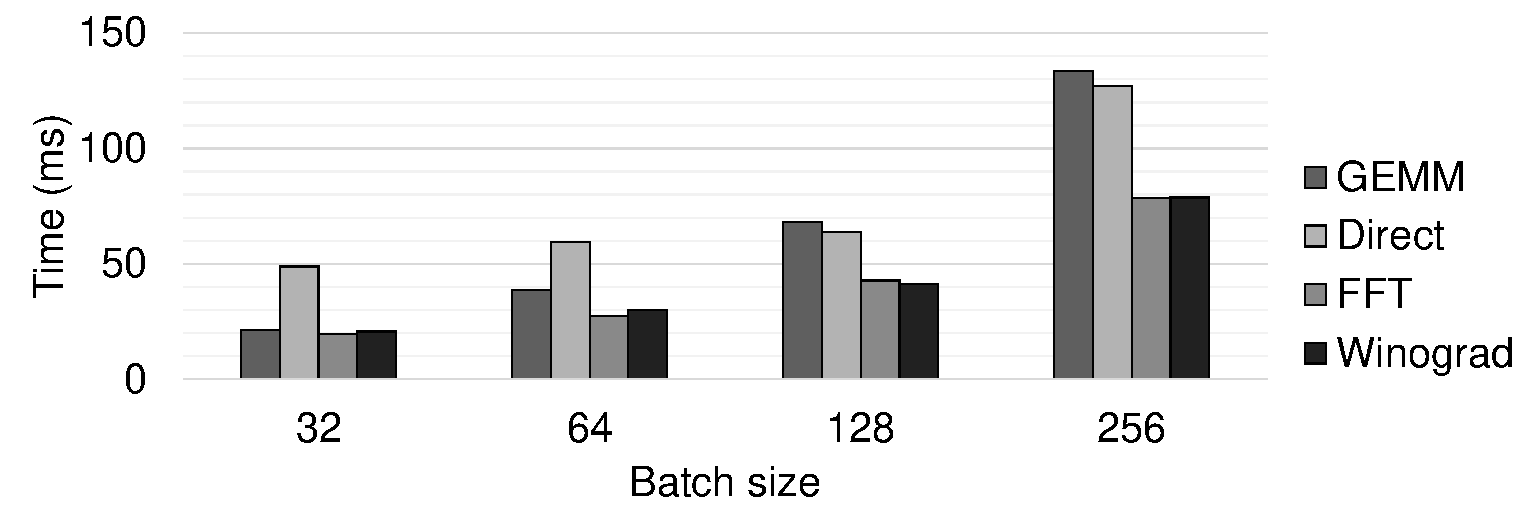
\includegraphics[width=.45\linewidth]{./figures/gpu_time_fwd}
  \label{fig_gpu_time_fwd}}
  \subfloat[Backpropagation execution time] {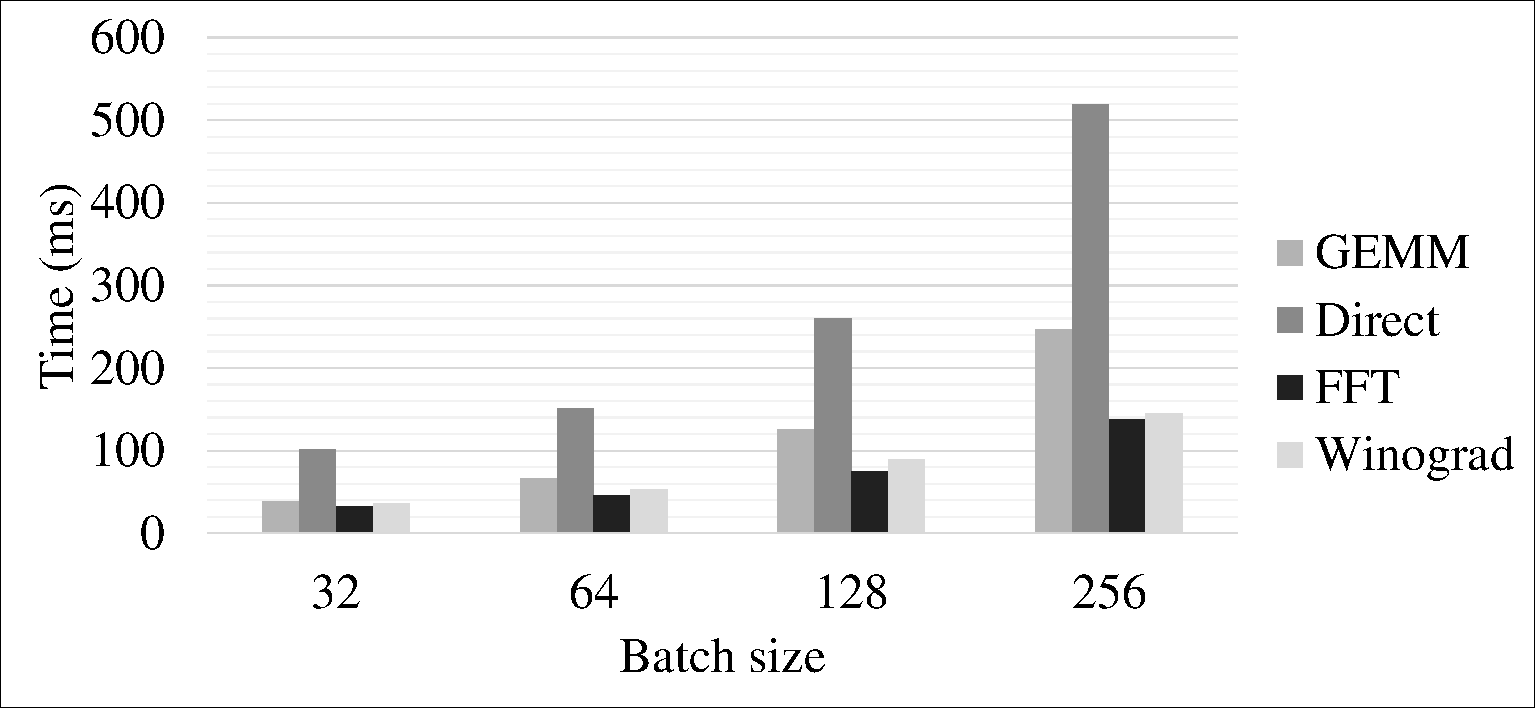
\includegraphics[width=.45\linewidth]{./figures/gpu_time_bwd}
  \label{fig_gpu_time_bwd}}
  \hfil
  \subfloat[Forward execution time from conv3 to conv5 layer] {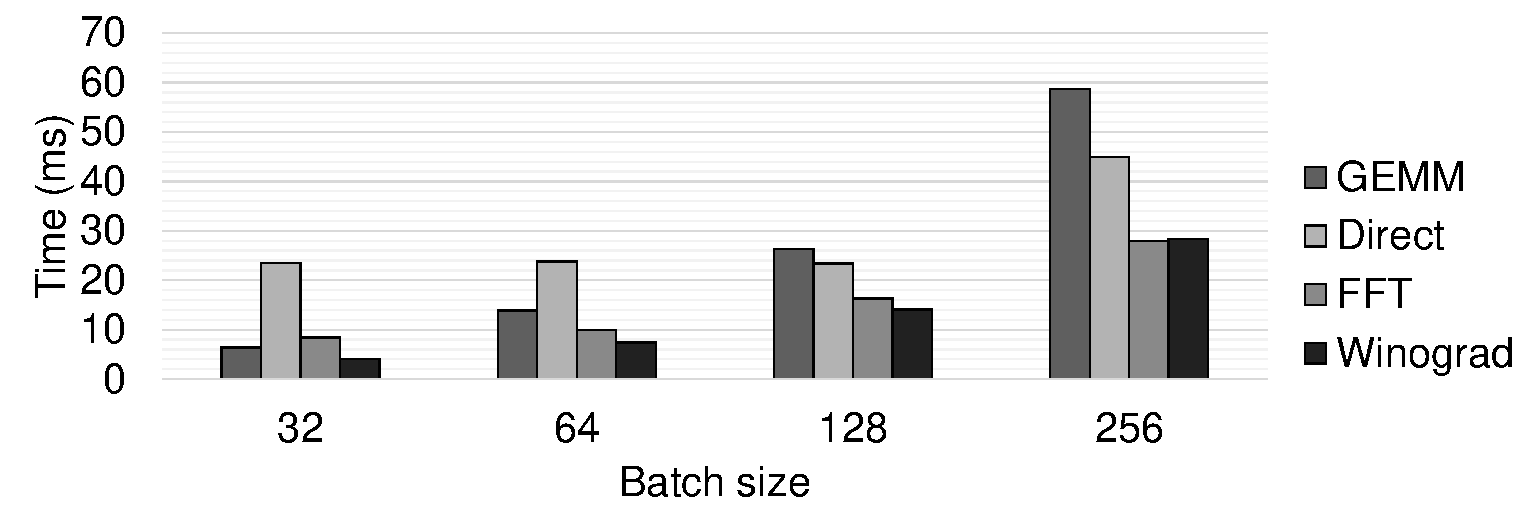
\includegraphics[width=.45\linewidth]{./figures/gpu_time_conv345}
  \label{fig_gpu_time_conv345}}
  \subfloat[Memory usage] {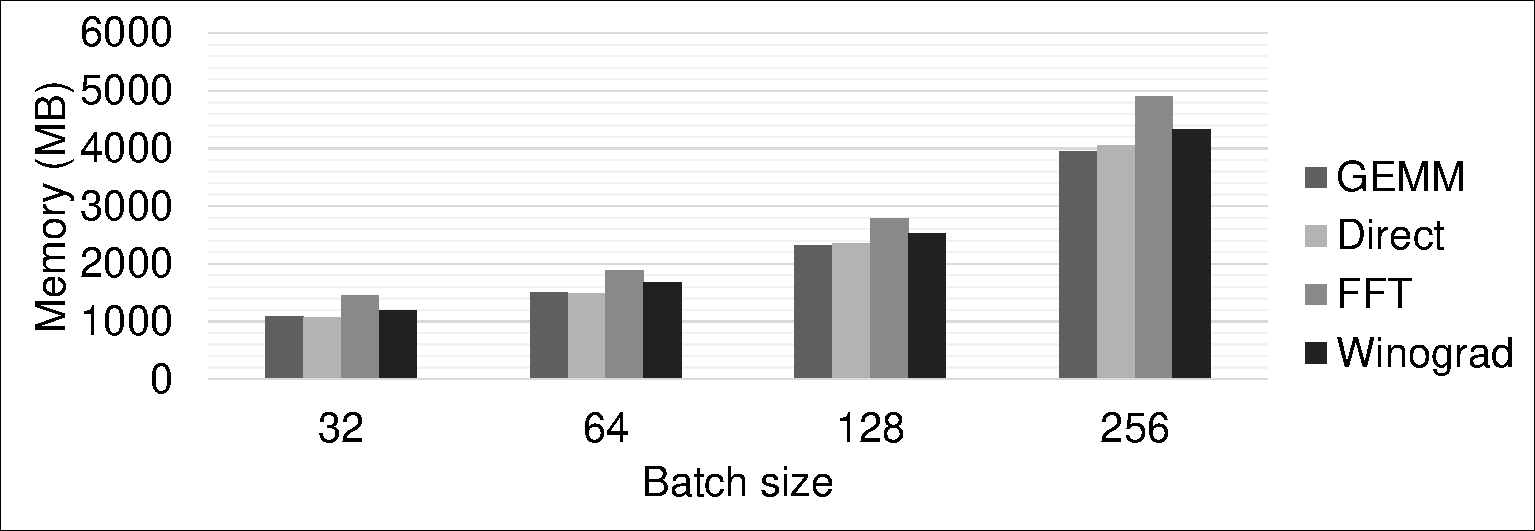
\includegraphics[width=.45\linewidth]{./figures/gpu_mem_kernels}
  \label{fig_gpu_mem}}
  \caption{Execution time and memory usage comparison of convolution kernels.}
  \label{fig_conv_time}
\end{figure*}

FIg \ref{fig_conv_time} shows execution time comparisons between convolution kernels.
The forward and backward propagation time is measured as average of 100 iterations.
Winograd convolution and FFT convolution perform better than direct or gemm convolution most of the time.
Since many recent CNN models use 3x3 filter for convolution layers\cite{vgg}, the forward propagation times of convolution layer 3 to 5 are separately tested and the result is on Fig \ref{fig_gpu_time_conv345}.
With respect to total training time, FFT is the fastest among all batch sizes.
But for 3x3 convolution layers, Winograd convolution performs better on smaller batch sizes.
Winograd convolution performs better on small batch sizes, while FFT scales better on bigger batch sizes.
Cuda-convnet scales bad when the batch size is smaller than 128 while GEMM convolutoin sclaes almost linearly.
Theoretically forward and backward propagation are symmetric.
Since backpropagation executes 2 convolutions per layer, the backpropagation time should be a double of forward propagation time.
While most other algorithms follow this rule, direct convolution kernels do not.
Backpropagation execution time of direct convolution is around a quadruple of forward propagation time.
Fig \ref{fig_gpu_mem} shows peak GPU device memory usage for each convolution algorithms.
FFT convolution kernels occupies the most GPU memory, using around 20\% more memory than GEMM convolution kernels.

\begin{figure*}[!t]
  \centering
  \subfloat[Forward execution time] {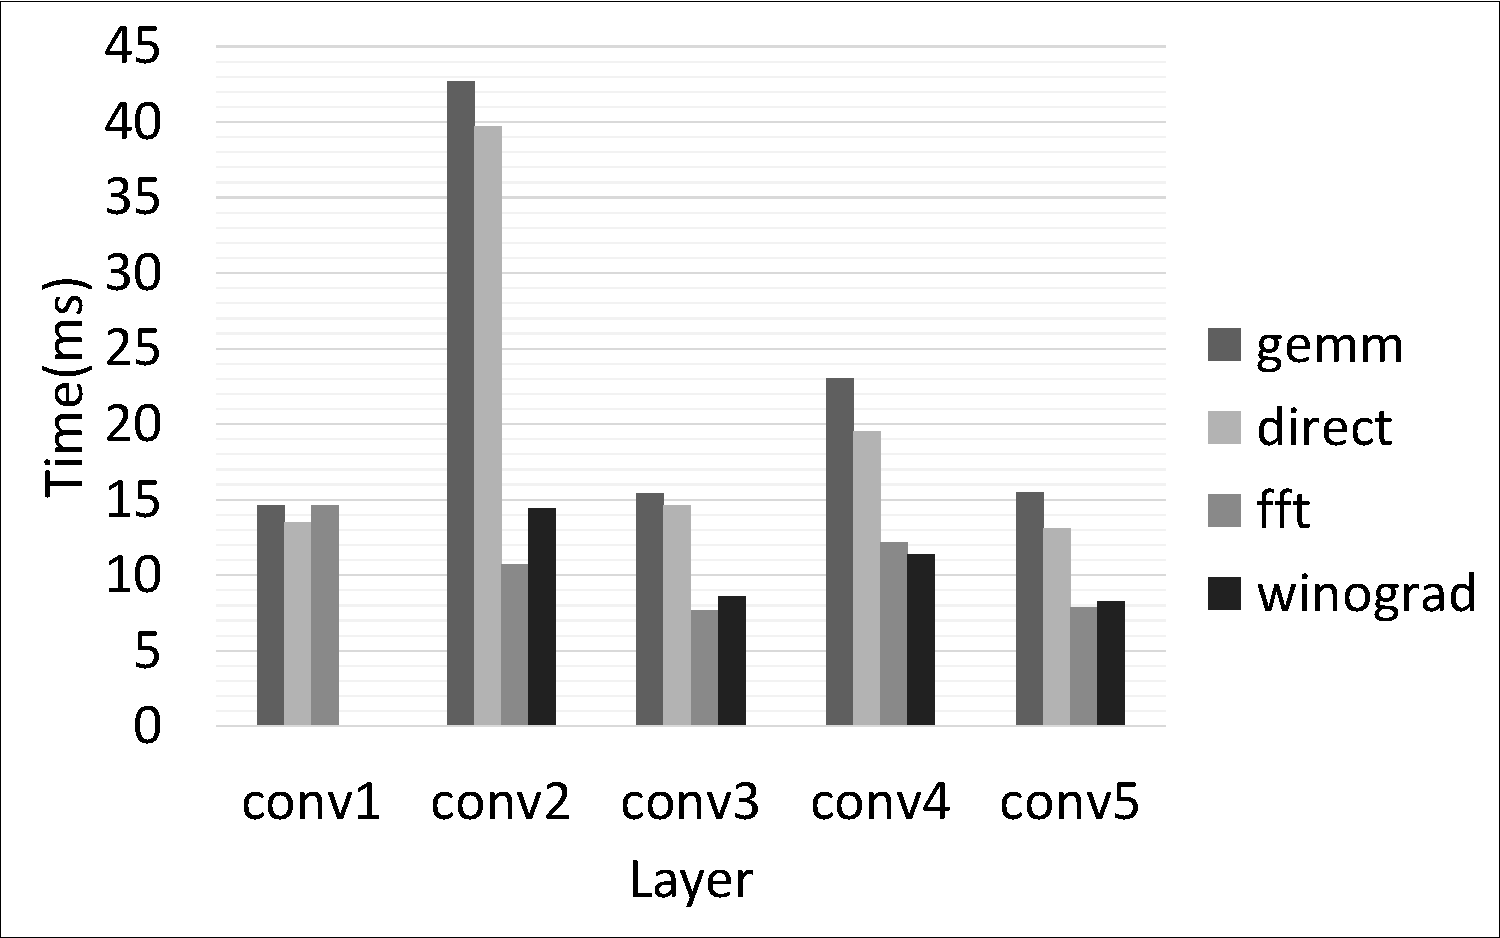
\includegraphics[width=.3\linewidth]{./figures/layerwise_fwd}
  \label{fig_layerwise_fwd}}
  \subfloat[Backward Data execution time] {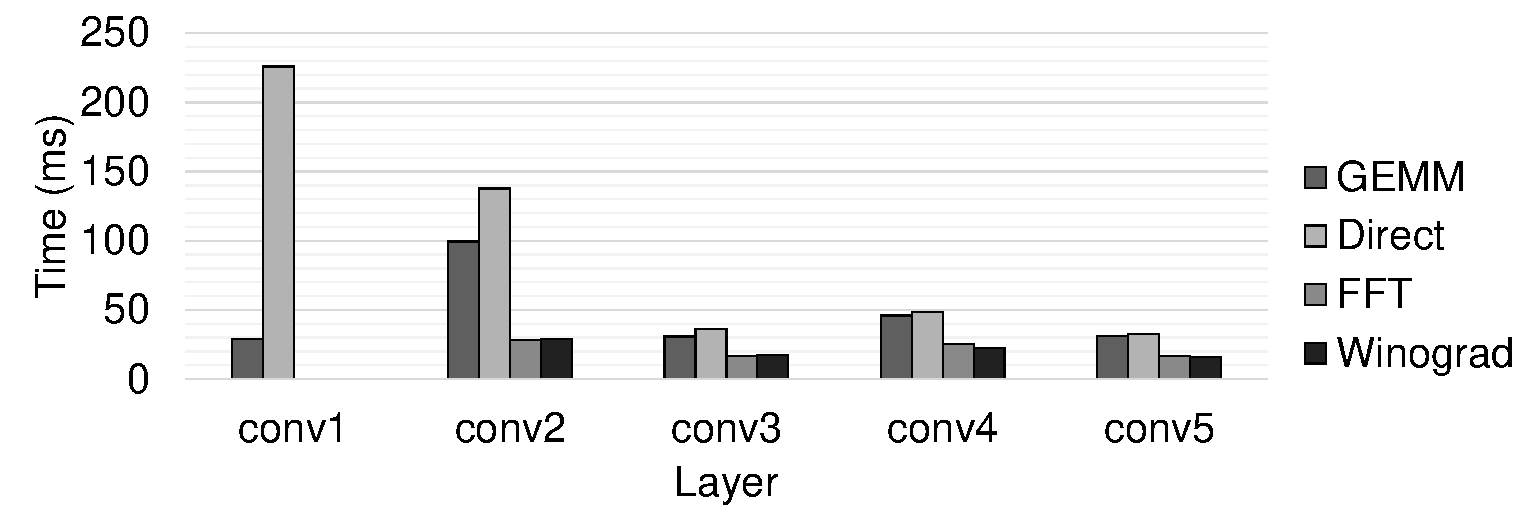
\includegraphics[width=.3\linewidth]{./figures/layerwise_bd}
  \label{fig_layerwise_bd}}
  \subfloat[Backward Filter execution time] {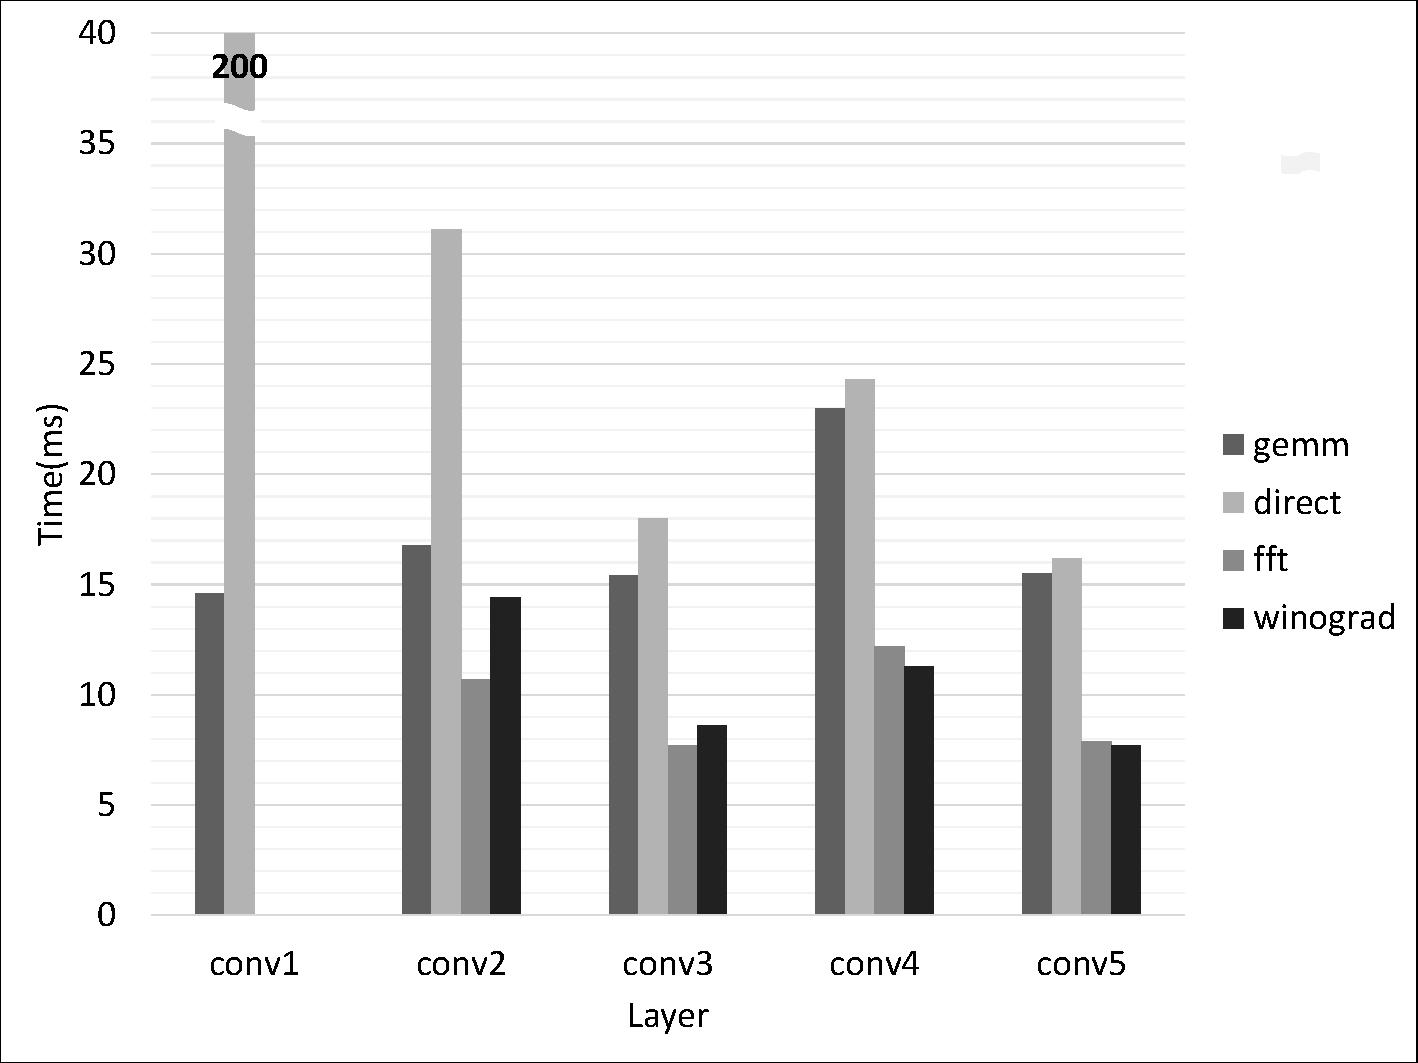
\includegraphics[width=.3\linewidth]{./figures/layerwise_bw}
  \label{fig_layerwise_bw}}
  \hfil
  \subfloat[Forward floating point operations count] {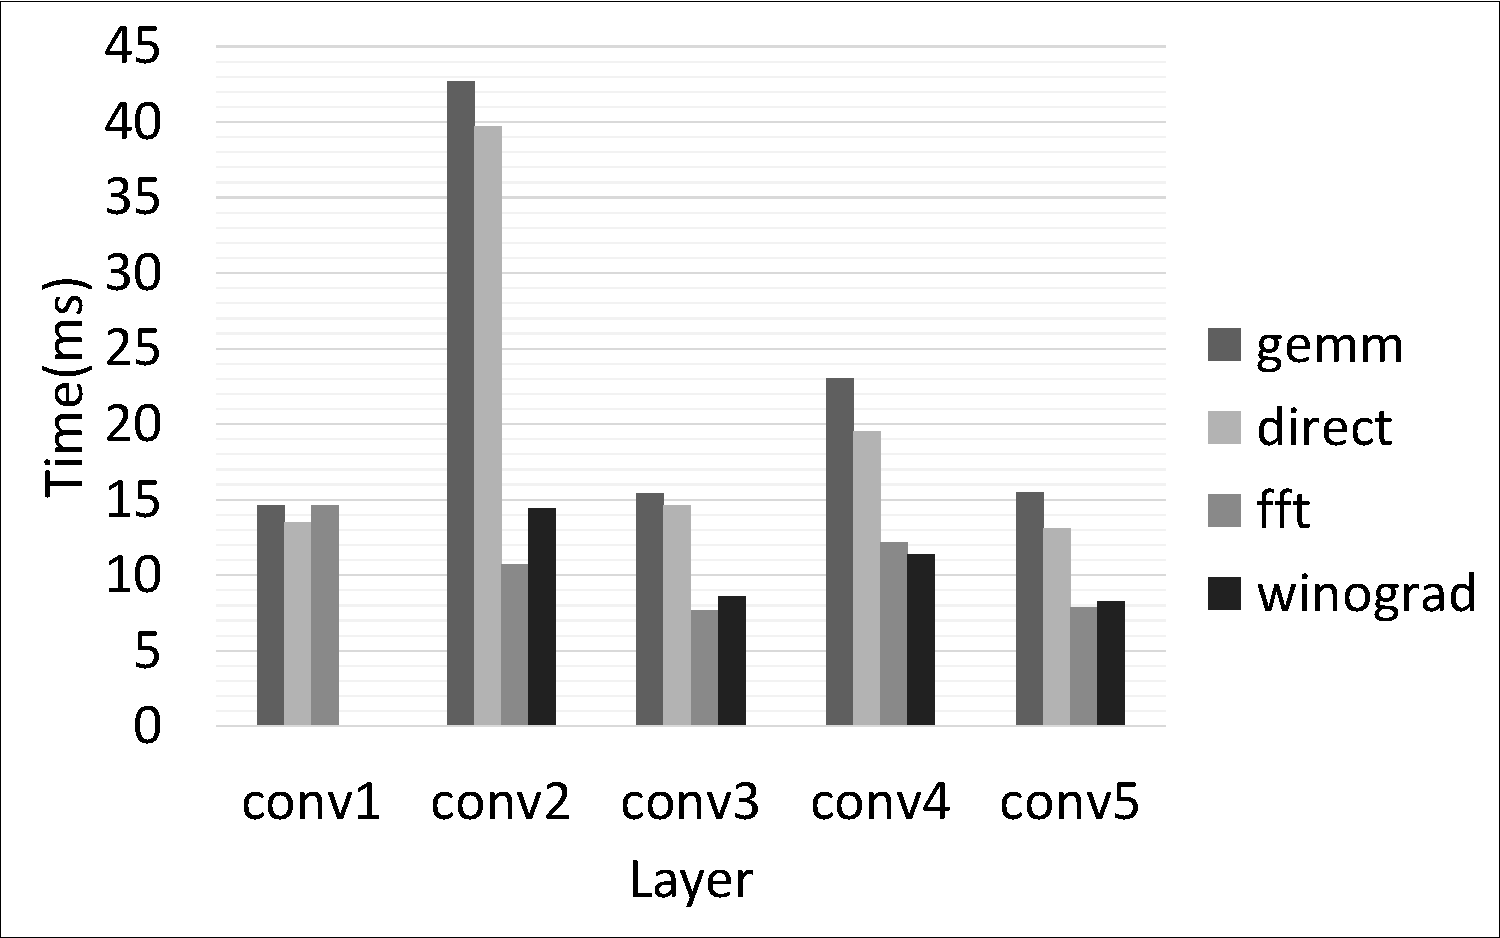
\includegraphics[width=.3\linewidth]{./figures/layerwise_fwd}
  \label{fig_layerwise_flop_count}}
  \subfloat[Forward Flops throughput] {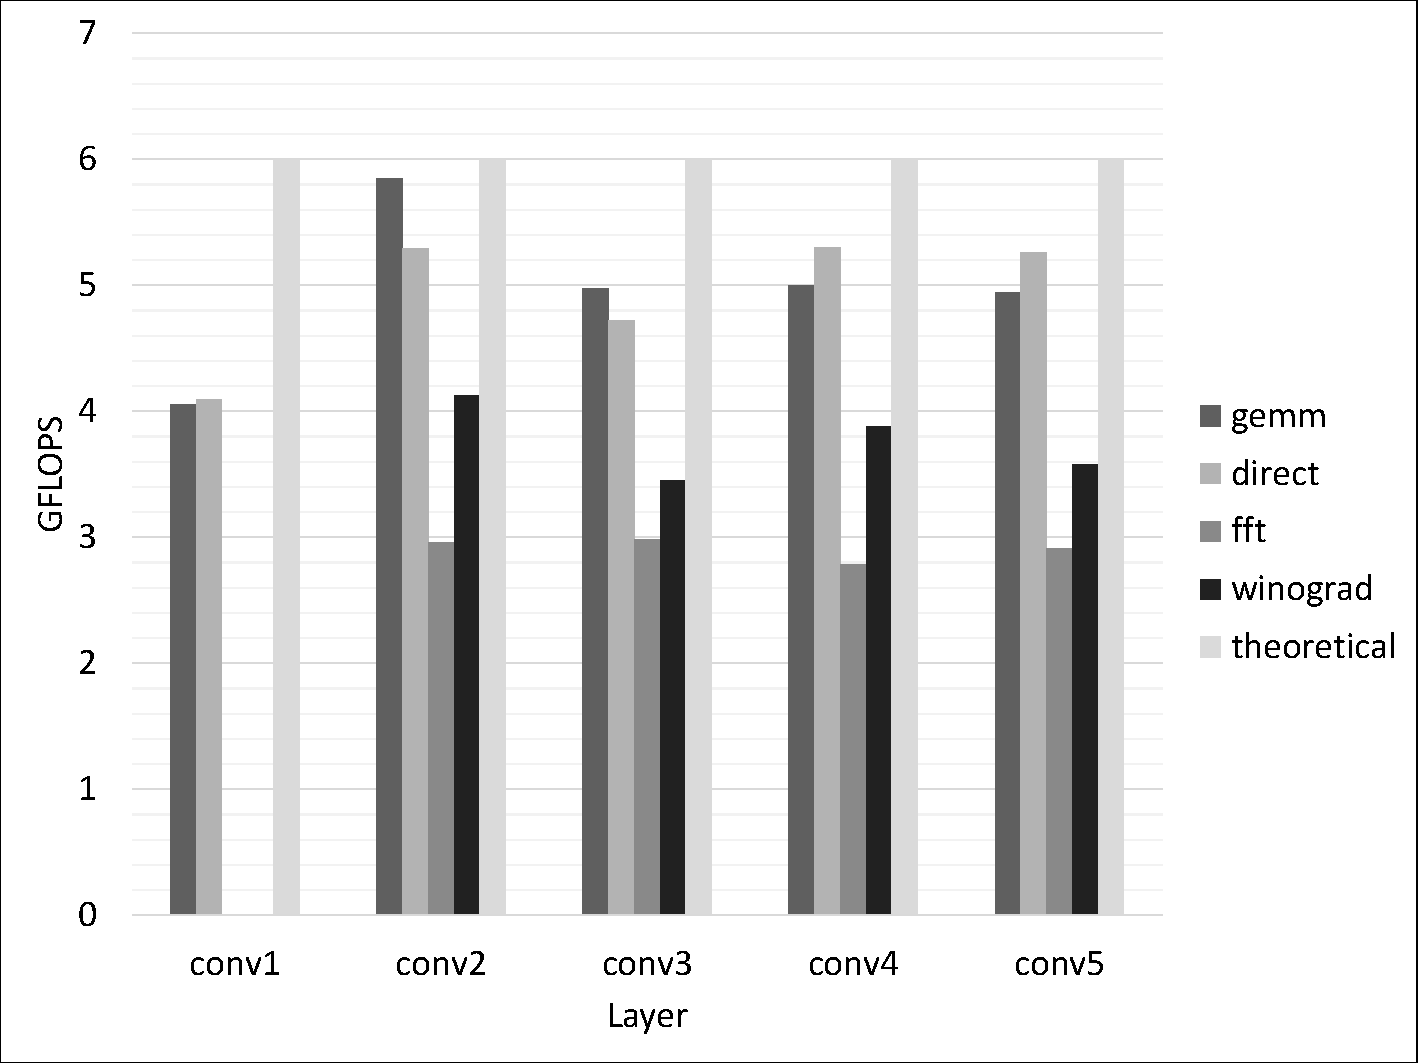
\includegraphics[width=.3\linewidth]{./figures/layerwise_flops_fwd}
  \label{fig_layerwise_flops_fwd}}
  \subfloat[Backward Flops throughput] {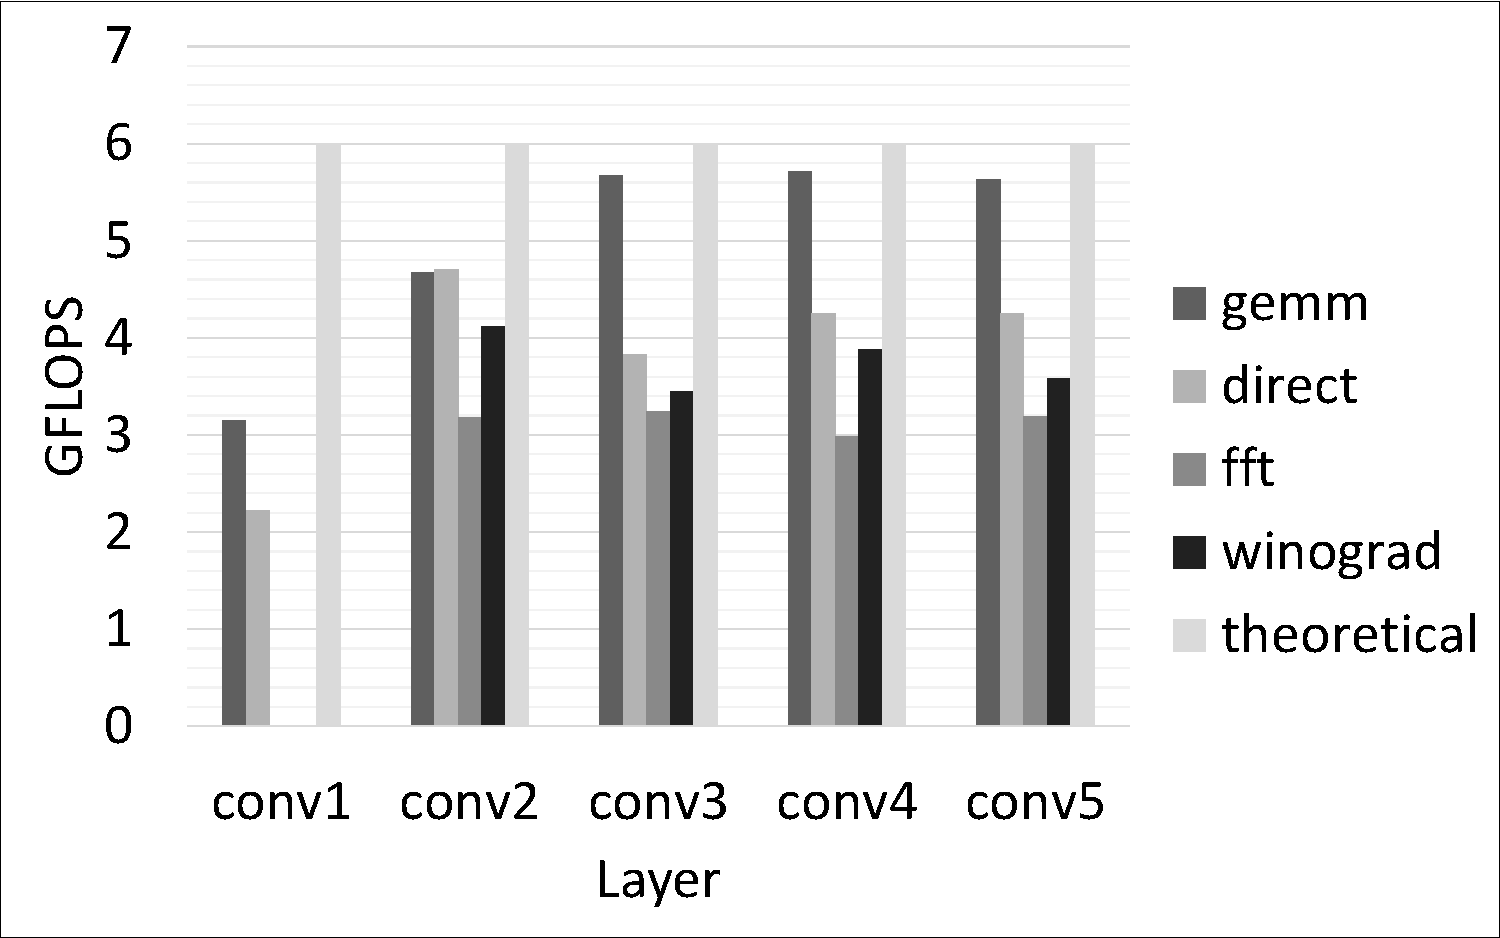
\includegraphics[width=.3\linewidth]{./figures/layerwise_flops_bd}
  \label{fig_layerwise_flops_bd}}
  \caption{Layerwise analysis of convolution kernels}
  \label{fig_layerwise}
\end{figure*}

Fig \ref{fig_layerwise} shows layerwise analysis of convolution algorithms.
The batch size for layerwise comparison is set to 256.
The compute times and statistics of kernels are measured by NVIDIA nvprof profiler.
The main performance limiter for backpropation of Cuda-convnet is backward filter convolution on conv1 layer.
We expect that reason for the slow execution is low parallelism of kernels.
The backward direct convolution kernels have small thread numbers compared to other algorithms, generating 6 times smaller thread grid size.
The backward filter convolution for the first layer generates only 1024 threads, while Titan X has 3072 CUDA cores.

FIg \ref{fig_layerwise_flop_count} compares floating operation counts of the convolution kernels measured by Nvidia's Cuda profiler.
The theoretical floating point operation counts are calculated as 2 * K*CRR*NWW since each calculation uses 1 addition and 1 multiplication.
FFT convolution consists of 1 filter flip kernel, 2 FFTs and 1 complex GEMM kernel.
Similarily nonfused Winograd convolution consists of 3 Tiling kernels and 36(in case of 3x3 filter) or 167(in case of 5x5 filter) GEMM kernels.
The statistics of those kernels are added up together per layer for the result.
Flops throughputs of the kernels shown in Fig \ref{fig_layerwise_flops_fwd} and Fig \ref{ fig_layerwise_flops_bd} are calculated as Flop count/execution time.
Compared to maximum Flops throughput of Nvidia TitanX is 6TFlops, most convolution kernels show throughput more than 3TFlops.
The Flops throughput result indicate that convolution kernels are compute bounded rather than memory.
Even if FFT has slower Flops throughput, FFT convolution is usually the fastest due to much less algorithm complexity.
Especially on convolution layer 2 which uses 5x5 filter for convolution, FFT convolution is much faster than other algorithms becuase computation complexity of FFT does not depend on filter sizes.
Winograd's filtering algorithm also reduces Flop count by more than half makes perform similar to FFT convolution on convolution layers with 3x3 filters.

\subsection{Multi GPU analysis}

\begin{itemize}
  \item Support
  \item Scalability : proportion of data exchange
  \item Synchronization cost
\end{itemize}
